\documentclass[]{article}

\usepackage[utf8]{inputenc}
\usepackage[usenames,dvipsnames]{xcolor}
\usepackage{fullpage}
\usepackage[upright]{fourier}
\usepackage{tkz-graph}
\usepackage{color}
\usetikzlibrary{arrows}

\usepackage[paperheight=2.3in,paperwidth=2.6in,margin=0in]{geometry}
\definecolor{color1}{RGB}{251,180,174}
\definecolor{color2}{RGB}{179,205,227}
\definecolor{color3}{RGB}{204,235,197}
\definecolor{color4}{RGB}{222,203,227}

\begin{document}
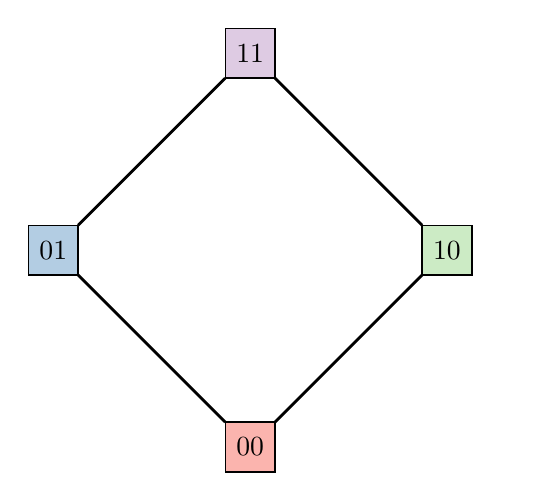
\begin{tikzpicture}
% reticulado booleano particionado com S' sendo a primeira e a segunda
% característica
  \SetVertexNormal[Shape     = rectangle,
                   FillColor = white,
                  LineWidth  = 1pt]
  \SetUpEdge[lw         = 1pt,
             color      = black,
             labelcolor = white,
             labeltext  = red,
             labelstyle = {sloped,draw,text=blue}]

%part 00
\SetVertexNormal[Shape = rectangle, FillColor  = color1]
\Vertex[x=0, y=0, LabelOut=true, Ldist=5pt]{}
\Vertex[x=0, y=0]{$00$}

%part 01
\SetVertexNormal[Shape = rectangle, FillColor  = color2]
\Vertex[x=-2.5, y=2.5, LabelOut=true, Ldist=5pt]{}
\Vertex[x=-2.5, y=2.5]{$01$}

%part 10
\SetVertexNormal[Shape = rectangle, FillColor  = color3]
\Vertex[x=2.5, y=2.5, LabelOut=true, Ldist=5pt]{}
\Vertex[x=2.5, y=2.5]{$10$}

% part 11
\SetVertexNormal[Shape = rectangle, FillColor  = color4]
\Vertex[x=0, y=5, LabelOut=true, Ldist=5pt]{}
\Vertex[x=0, y=5]{$11$}

\tikzset{EdgeStyle/.style={-}}

% part 00
\SetUpEdge[lw = 1pt, color= black]
\Edges($00$, $01$) 
\Edges($00$, $10$) 
\Edges($01$, $11$) 
\Edges($10$, $11$) 

\end{tikzpicture}
\end{document}
